\section{Correlations by Problem Difficulty}
\subsection{Problem Difficulty vs. Correctness Checking} \label{appendix:difficulty-correctness-full}
In Fig. \ref{fig:correctness-checking-difficulty-all}, we show the accuracy of HumanEval (top), LeetCode (middle), and ODEX (bottom) across different models. We see an absence of correlation across the board.

\begin{figure}[H]
    \centering
    \begin{subfigure}[b]{\textwidth}
        \centering
        
\includegraphics[width=\linewidth]{figures_v2/appendix/difficulty_barplots/humaneval_correctness.pdf}
        % \subcaption{HumanEval}
    \end{subfigure}
\end{figure}
\begin{figure}[H] 
    \ContinuedFloat
    \centering
    \begin{subfigure}[b]{0.5\textwidth}
        \centering
        
\includegraphics[width=\linewidth]{figures_v2/appendix/difficulty_barplots/livecodebench_correctness.pdf}
        % \subcaption{LeetCode}
    \end{subfigure}
    \begin{subfigure}[b]{0.9\textwidth}
        \centering
        
\includegraphics[width=\linewidth]{figures_v2/appendix/difficulty_barplots/odex_correctness.pdf}
        % \subcaption{ODEX}
    \end{subfigure}
    \caption{Accuracies for correctness checking task bucketed by difficulty.}
    \label{fig:correctness-checking-difficulty-all}
\end{figure}

\subsection{Problem Difficulty vs. Execution} \label{appendix:difficulty-execution-full}

In Fig. \ref{fig:execution-difficulty-all}, we show the accuracy of HumanEval (a), LeetCode (b), and ODEX (c) across different models. We see a slight correlation, where programs for more difficult problems are harder to execute.

\begin{figure}[H]
    \centering
    \begin{subfigure}[b]{\textwidth}
        \centering
        
\includegraphics[width=\linewidth]{figures_v2/appendix/difficulty_barplots/humaneval_execution.pdf}
        \subcaption{HumanEval}
    \end{subfigure}
\end{figure}
\begin{figure}[H]
    \ContinuedFloat
    \centering
    \begin{subfigure}[b]{0.5\textwidth}
        \centering
        
\includegraphics[width=\linewidth]{figures_v2/appendix/difficulty_barplots/livecodebench_execution.pdf}
        \subcaption{LeetCode}
    \end{subfigure}
    \caption{Accuracies for execution task bucketed by difficulty.}
    \label{fig:execution-difficulty-all}
\end{figure}

\clearpage
\subsection{HumanEval Pass Rate vs. Correctness Prediction}
In Fig. \ref{fig:pass-rate-cm}, we investigate the correlation between a program's pass rate on HumanEval (using EvalPlus tests) and its prediction. Since a problem's pass rate is indicative of how close it is to correct, we might expect that programs with a higher pass rate have a higher chance of being predicted as correct. For most models, this does not seem ot be the case, though we do see this trend for GPT-4.

\begin{figure}[H]
    \centering
    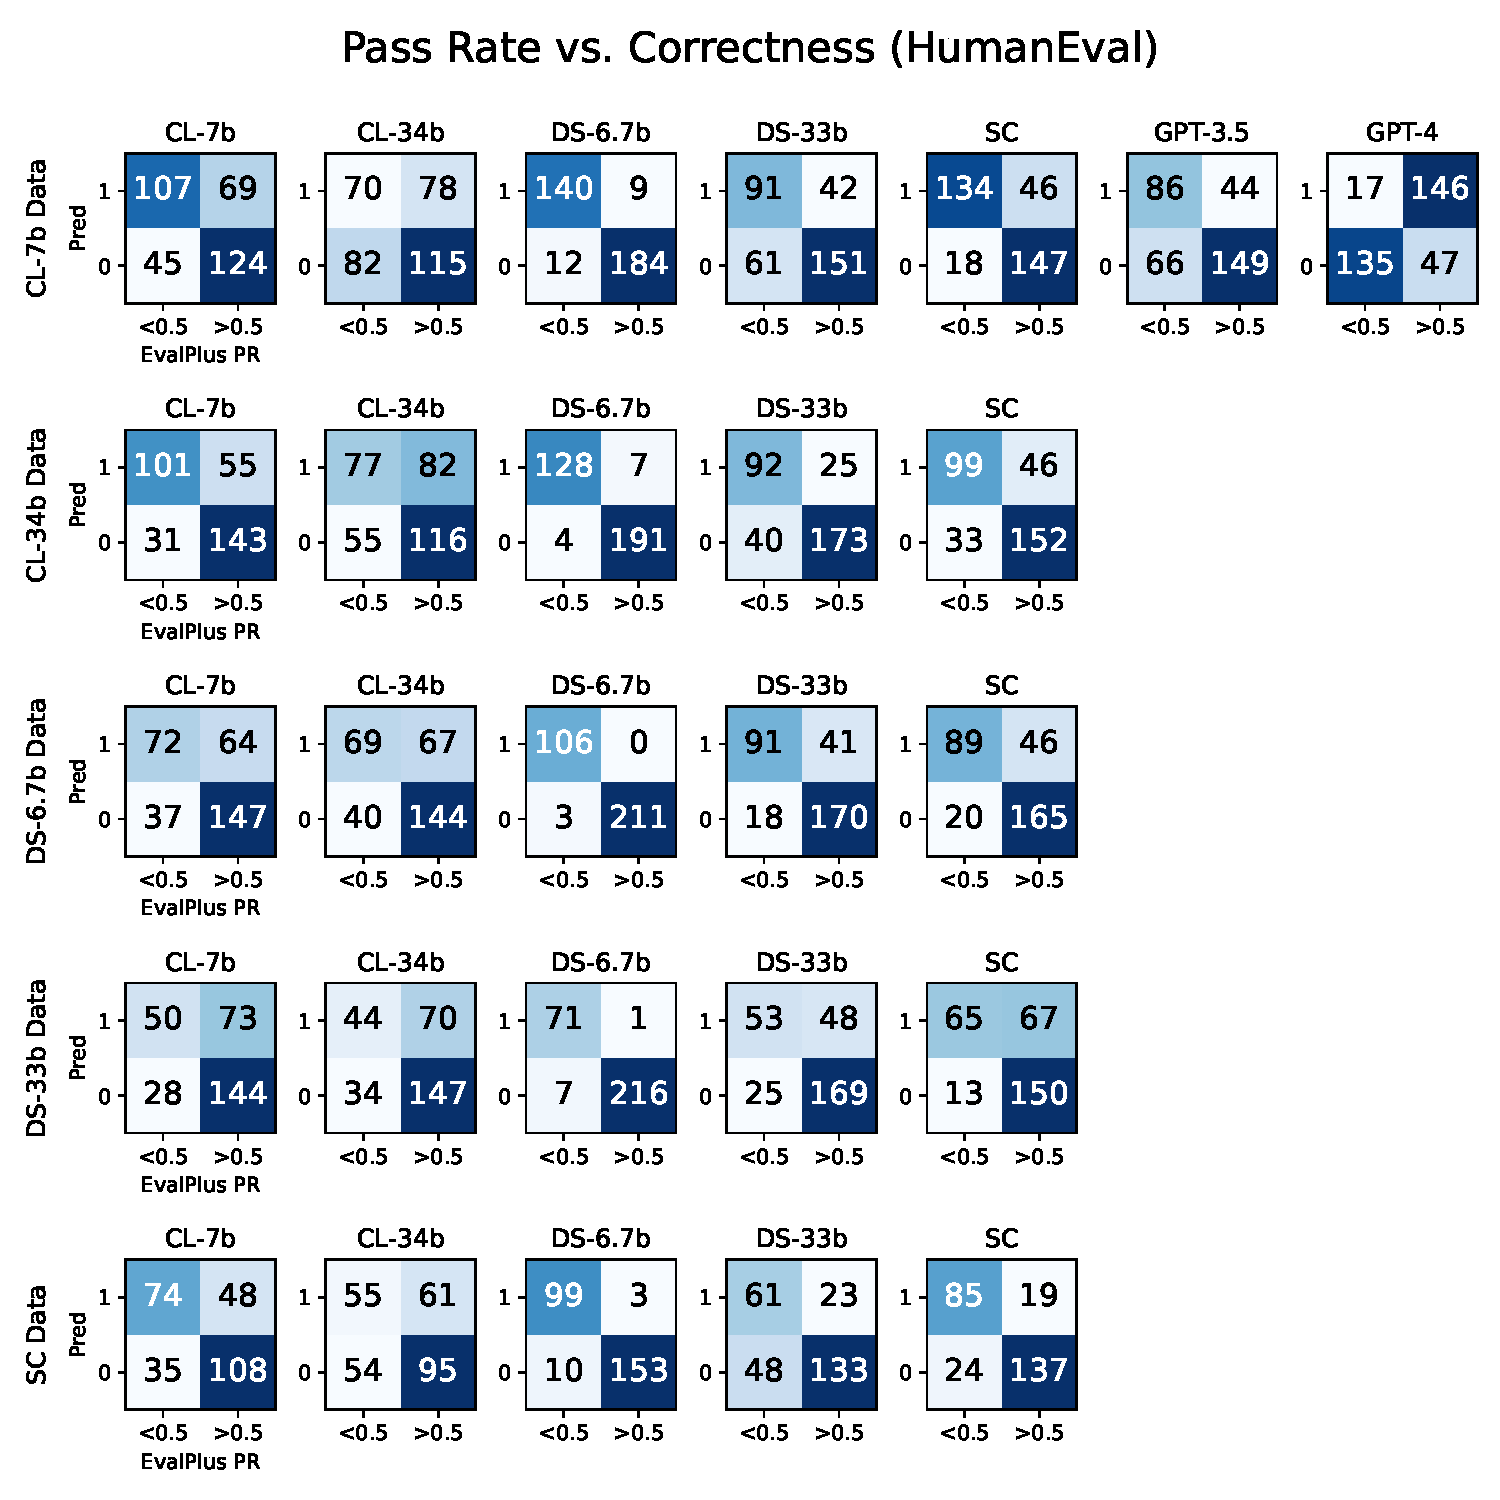
\includegraphics[width=\linewidth]{figures_v2/appendix/accuracy_correlations/humaneval_cm.pdf}
    \caption{Models other than GPT-4 show a lack of correlation between a problem's pass rate and its correctness prediction.}
    \label{fig:pass-rate-cm}
\end{figure}